% chap2.tex (Definitions)

\chapter{Anatom\'ia de los huesos y fracturas}

Los huesos son \'organos compuestos de tejido vivo duro que realizan muchas funciones incluyendo el soporte estructural de nuestro cuerpo. Dentro del cuerpo humano, los huesos se encuentran clasificados de diferentes formas, tanto desde el punto de vista macrosc\'opico como microsc\'opico. A pesar de su dureza, la fractura de huesos ocurre con frecuencia. Estas fracturas necesitan ser diagnosticadas y tratadas por un m\'edico traumat\'ologo. El m\'edico traumat\'ologo necesita determinar el tipo de fractura y el tratamiento a emplear para un paciente con la lesi\'on.

En el presente cap\'itulo, se examinar\'a la estructura y funci\'on de los huesos as\'i como la clasificaci\'on de las fracturas y su tratamiento.

\section{Estructura del hueso}

El esqueleto humano (Figura \ref{fig:skeleton}) est\'a compuesto por 206 huesos, los cuales representan alrededor del 20\% de la masa corporal. Los huesos son un tipo de tejido duro conectivo endoesquel\'etico que soportan la estructura del cuerpo, protegen los \'organos internos (como el cerebro, m\'edula espinal y \'organos del t\'orax) y facilitan el movimiento junto a otros tejidos (los tendones, ligamentos y m\'usculos).
\begin{figure}[htb]
	\centering
		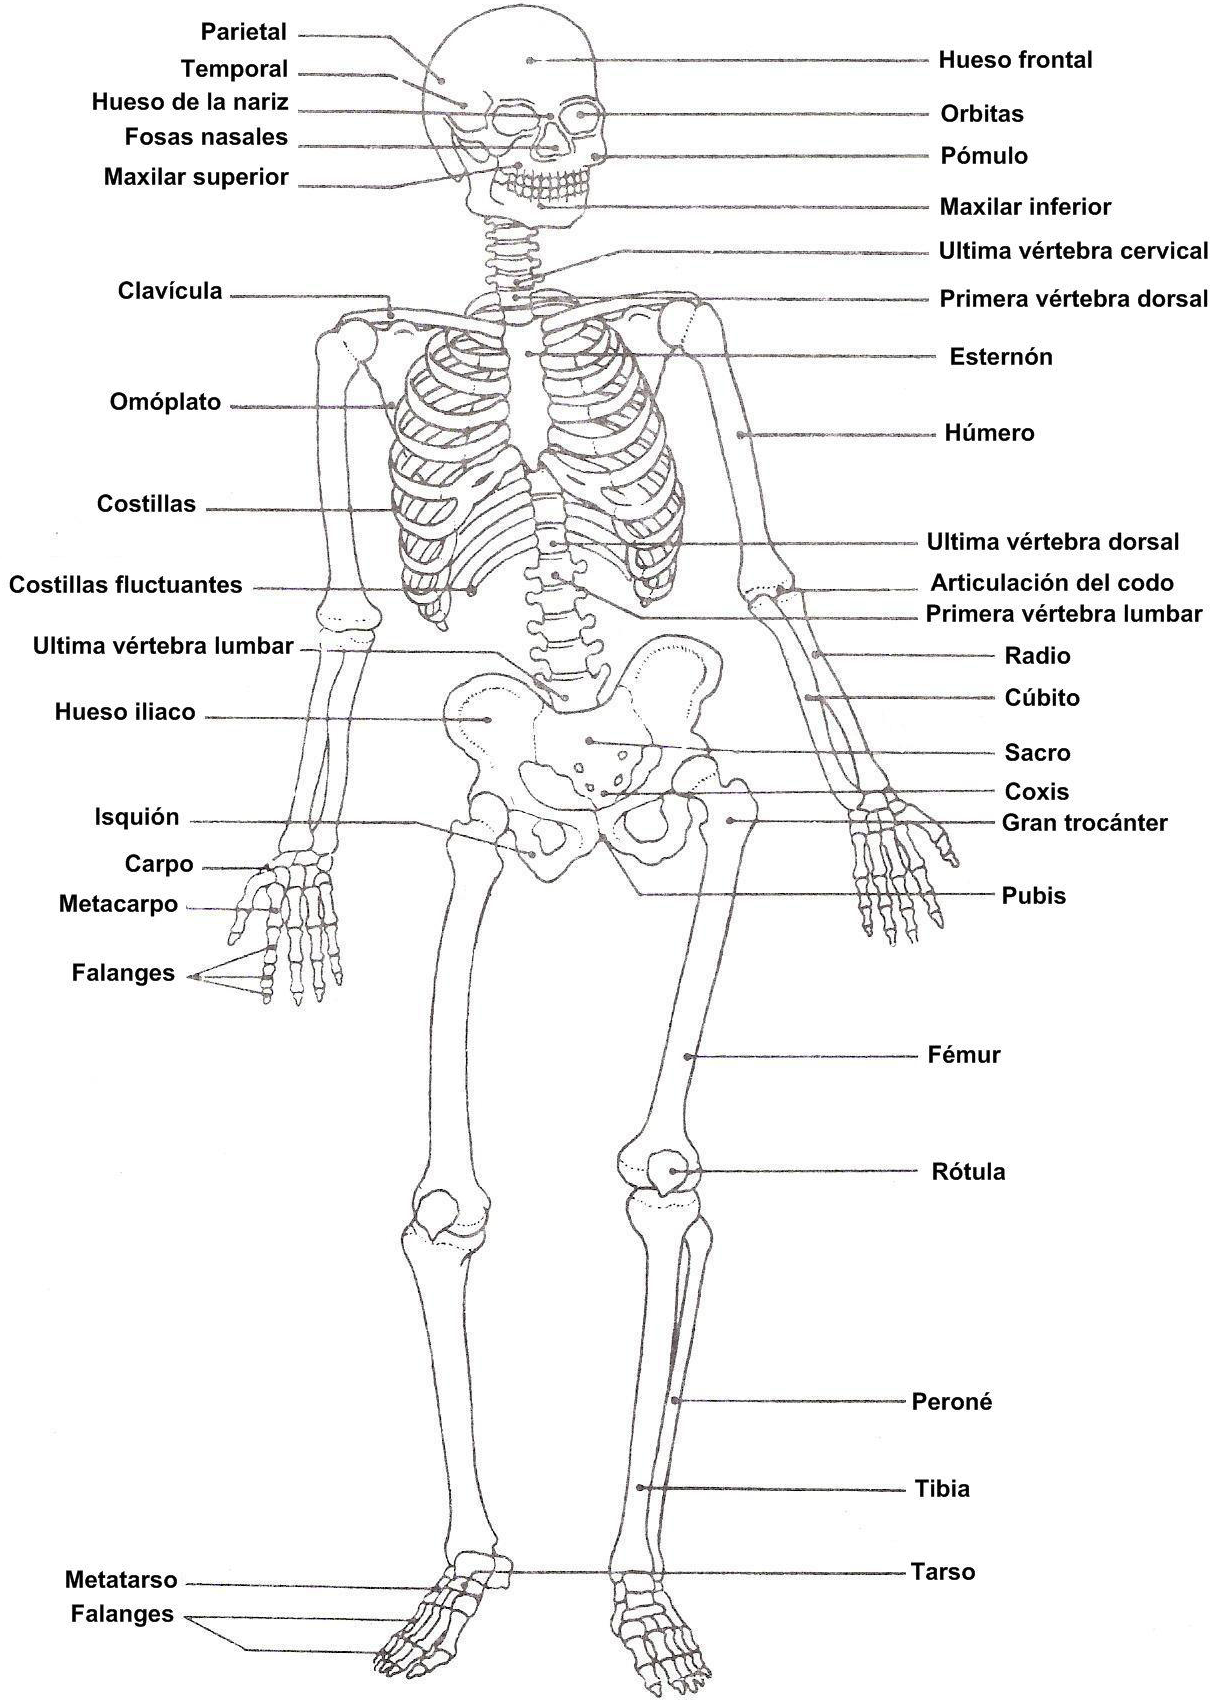
\includegraphics[width=0.35\columnwidth]{images/skeleton.png}
		\caption{Huesos del cuerpo humano}
	\label{fig:skeleton}
\end{figure}

Un hueso est\'a compuesto por un material duro y liviano que contiene componentes org\'anicos e inorg\'anicos formados por c\'elulas vivas dentro de un conjunto org\'anico mineralizado. Los componentes org\'anicos incluyen las c\'elulas (osteoblastos, osteocitos y osteoclastos) y la matriz osteoide. Los componentes org\'anicos, son los responsables de la flexibilidad y tensi\'on que permiten al hueso resistir la torsi\'on y el estiramiento. Sin estos componentes, los huesos seguir\'ian siendo duros pero muy fr\'agiles.

Por otra parte, los componentes inorg\'anicos del hueso representan el 65\% de la masa del mismo, y est\'an formados por microesferas de hidroxiapatita de calcio. Este componente permite obtener una excepcional dureza del hueso. La combinaci\'on de los componentes org\'anicos e inorg\'anicos permiten que los huesos posean caracter\'isticas como durabilidad y dureza sin llegar a ser fr\'agiles.

%%%%%%%%%%%%%%%%%%%%%%%%%%%%%%%%%%%%%%%%%%%%%%%%%%%%%%%%
\subsection{Tipos de hueso}

Un hueso puede ser clasificado por la estructura que posee o por su forma. A continuaci\'on se describen estas dos clasificaciones.

\subsubsection*{Clasificaci\'on por Estructura}

Los huesos tienen una estructura interna en forma de un mallado que var\'ia en cuanto a su densidad en diferentes zonas. La estructura de un hueso puede ser compacta o esponjosa como se muestra en la Figura \ref{fig:esponjosocompacto}. Por ejemplo, la capa externa del hueso cortical es de estructura compacta y comprime una porci\'on importante de masa esquel\'etica. Una estructura esponjosa, se puede observar en el hueso trabecular donde su estructura es similar a un panal de abejas.
\begin{figure}[htb]
	\centering
		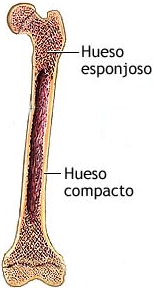
\includegraphics[width=0.20\columnwidth]{images/esponjosocompacto.png}
		\caption{Clasificaci\'on de huesos por su estructura}
	\label{fig:esponjosocompacto}
\end{figure}

\subsubsection*{Clasificaci\'on por Forma}

Los huesos pueden ser clasificados por su forma como largos, cortos, planos o irregulares, como se muestra en la Figura \ref{fig:byshape}. Los huesos largos como el f\'emur, ver Figura \ref{fig:byregion}, son estructuras tubulares que consisten en las siguientes regiones:

\begin{figure}[htb]
  \begin{center}
 \subfigure[]{\label{fig:byshape}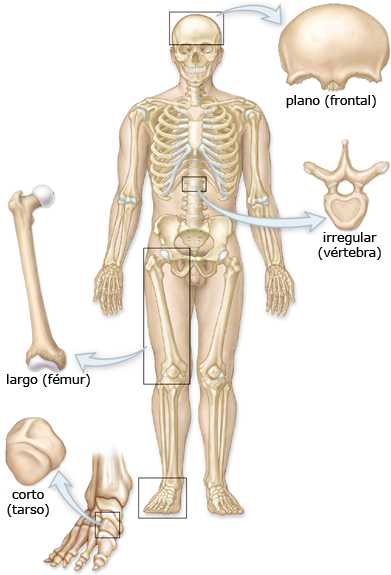
\includegraphics[width=0.40\columnwidth]{images/boneByShape.png}} \hspace{1cm}
    \subfigure[]{\label{fig:byregion}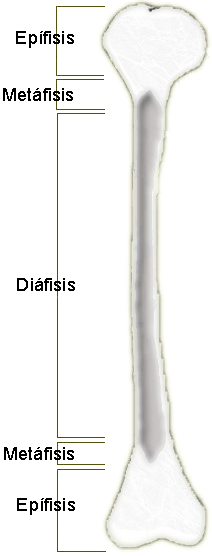
\includegraphics[scale=0.35]{images/femur1.png}}
  \end{center}
  \caption{(a) Clasificaci\'on de huesos por su forma.(b) Regiones de los huesos largos}
  \label{fig:second}
\end{figure}

\subparagraph{Di\'afisis:}El eje central de un hueso largo es llamado di\'afisis. Est\'a localizada entre las met\'afisis y consiste de una pared de hueso compacto y tiene una cavidad hueca medular rellena de m\'edula \'osea. La superficie externa de la di\'afisis est\'a cubierta por el periostio.

\subparagraph{Met\'afisis:}Es una zona intermedia ubicada entre la ep\'ifisis y la di\'afisis. Las placas epifisarias (i.e. placas de crecimiento) se encuentran en las met\'afisis y son responsables del crecimiento y el alargamiento de los huesos durante la infancia.

\subparagraph{Ep\'ifisis:}Est\'a constituida por los 2 extremos del hueso en los que se encuentran las superficies articulares del hueso. Consiste en su mayor\'ia de hueso esponjoso cubierto por una capa relativamente delgada de hueso compacto cortical.

Los huesos cortos, como los huesos de los dedos, la mu\~neca, los huesos del tobillo y la r\'otula, tienen una estructura similar a los huesos largos, excepto que no tienen cavidad medular. Los huesos planos del cr\'aneo y las costillas consisten en dos capas de hueso compacto con una zona de hueso esponjoso situado entre ellos. Por \'ultimo los huesos irregulares son los huesos como las v\'ertebras y la pelvis, que no encajan en ninguna de las categor\'ias anteriores. En el caso particular del f\'emur, \'este es el hueso tubular m\'as largo del cuerpo y est\'a rodeado por la masa muscular m\'as extensa.

%%%%%%%%%%%%%%%%%%%%%%%%%%%%%%%%%%%%%%%%%%%%%%%%%%%%%%
\section{Fractura del hueso}

A pesar de que son muy flexibles y fuertes, los huesos son susceptibles al da\~no. Si se aplica m\'as fuerza en un hueso del que puede soportar, \'este se quiebra. Una ruptura de cualquier tama\~no se conoce como una fractura. La mayor\'ia de las fracturas que se producen antes de la edad adulta son consecuencia de traumatismos excepcionales tales como lesiones deportivas, ca\'idas de altura, accidentes automovil\'isticos y ca\'idas que tuercen o aplastan los huesos.

Las fracturas de hueso se pueden originar por 3 causas principales:

\subparagraph{Traumatismo directo:}El foco de fractura ha sido producido por un golpe directo. La energ\'ia producida se transmite directamente por la piel y las partes blandas. Esta clasificaci\'on tambi\'en abarca las fracturas producidas como consecuencia de una ca\'ida, en las cuales el hueso es el medio de transmisi\'on de la acci\'on de la fuerza y el suelo (u otro elemento contundente), superando la resistencia \'osea.
\subparagraph{Traumatismo indirecto:}El punto de aplicaci\'on de la fuerza est\'a alejado del foco de fractura. En este caso, las fuerzas aplicadas tienden a torcer o angular el hueso. Por ejemplo, la ca\'ida desde una motocicleta, con rotaci\'on de la pierna, produce una fractura a nivel medio de la tibia y el peron\'e, estando las fuerzas aplicada a nivel del pie fijo y de todo el cuerpo en rotaci\'on y ca\'ida.
\subparagraph{Por fatiga:}La fuerza que origina la fractura es aplicada en forma prolongada e intermitente en el tiempo. Por ejemplo, la fractura de marcha que se produce en algunos atletas o reclutas del ej\'ercito, que se produce en el pie.
%\end{enumerate}

\subsection{Tipos}

Pueden ocurrir distintos tipos de fracturas y estas var\'ian de acuerdo a su impacto, van desde una l\'inea muy fina de fractura hasta una fractura compleja formada por dos o m\'as fragmentos de hueso. En una clasificaci\'on b\'asica, las fracturas se pueden clasificar como simples o multifragmentarias. El t\'ermino simple se emplea para describir una sola l\'inea de fractura de un hueso roto con las partes a\'un en su posici\'on anat\'omicamente normal y un da\~no m\'inimo al tejido circundante. Por otra parte, el t\'ermino multifragmentaria se utiliza cuando hay dos o m\'as fragmentos de hueso presente en la fractura. 

Las fracturas tambi\'en pueden describirse como abiertas (tambi\'en conocido como expuestas) y cerradas, como se muestra en la Figura \ref{fig:fracture1}. En una fractura abierta, un hueso roto sobresale al exterior del cuerpo a trav\'es de una herida abierta, dando lugar a lesiones de tejidos blandos de los m\'usculos, tendones, ligamentos, vasos sangu\'ineos y nervios. Con fracturas abiertas, existe un alto riesgo de infecci\'on de los tejidos internos. Una fractura cerrada es una fractura del hueso que se mantiene interna y generalmente se da en combinaci\'on con una lesi\'on de un \'organo, la arteria o nervios.
\begin{figure}[htb]
	\centering
		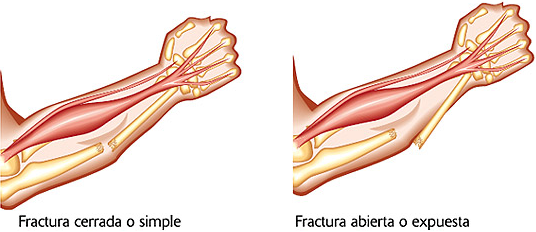
\includegraphics[width=0.60\columnwidth]{images/fractura1.png}
		\caption{Fractura cerrada y fractura abierta}
	\label{fig:fracture1}
\end{figure}

Las fracturas tambi\'en se pueden clasificar en otras categor\'ias: transversal, oblicua, espiral, alas de mariposa o conminuta (ver Figura \ref{fig:fracture2}). Este tipo de clasificaci\'on var\'ia de acuerdo a la forma de la ruptura del hueso y a sus caracter\'isticas: \'angulo, fractura del eje, zona del segmento de hueso, etc. Un tipo adicional de fractura es la fractura por insuficiencia. Las fracturas por insuficiencia son de dos tipos: por estr\'es y osteopor\'otico. Una fractura de estr\'es es una lesi\'on por uso excesivo causado por fuerzas repetitivas o prolongadas contra el hueso, causando una fisura a la forma. Estas fracturas son m\'as frecuentes en las extremidades inferiores como consecuencia de las fuerzas de reacci\'on del suelo en actividades como correr, caminar, marchar, o saltar. Por otro lado, las fracturas osteopor\'oticas son originadas por una enfermedad llamada osteoporosis, la cual disminuye la cantidad de minerales en el hueso, ocasionando la p\'erdida de fuerza en la parte del hueso trabecular y reduciendo la zona cortical por un defecto en la absorci\'on del calcio.

\begin{figure}[htb]
	\centering
		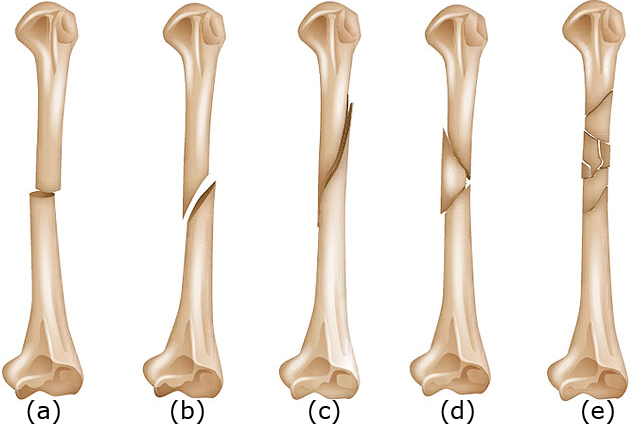
\includegraphics[width=0.50\columnwidth]{images/fracture2.png}
		\caption{Clasificaci\'on de fracturas (a) Transversal (b) Oblicuo (c) Espiral (d) Alas de Mariposa (e) Conminuta}
	\label{fig:fracture2}
\end{figure}

%begin check
\subsection{Incidencia}

En Venezuela, no existe un estudio poblacional del \'area de Salud para la incidencia de fracturas en la poblaci\'on. Una publicaci\'on realizada por el Dr. Strocchia et al. \cite{STRO01} en el a\~no 2001, refleja un estudio con 59 pacientes con el objetivo de evaluar las eventualidades surgidas con diversos m\'etodos de fijaci\'on. Strocchia et al. \cite{STRO01} realizaron el estudio en el Hospital Dr. Victorino Santaella Ru\'iz de Los Teques, en el per\'iodo de Enero 2001 hasta Diciembre 2001. En dicho estudio, se evidenci\'o una alta incidencia en pacientes j\'ovenes con predominio del sexo masculino ($81.35\%$), siendo las heridas por arma de fuego la principal causa ($38.9\%$).

En los Estados Unidos de Norteam\'erica, seg\'un la informaci\'on mostrada en \cite{NAT02}, durante el a\~no 2001 las fracturas representaron el $7,0\%$ del total de lesiones no fatales y enfermedades que motivaron d\'ias de ausencia al trabajo en ese a\~no. Esta categor\'ia incluye tanto fracturas abiertas como cerradas de huesos y dientes. Las fracturas se encuentran entre los problemas ortop\'edicos m\'as frecuentes \cite{DIS05}. Aproximadamente 6,8 millones de ciudadanos estadounidenses se fracturan un hueso al a\~no. En promedio, en los Estados Unidos de Norteam\'erica cada persona vive la experiencia de dos fracturas a lo largo de su vida.

En el caso particular de fractura del f\'emur, en los Estados Unidos de Norteam\'erica durante el a\~no 2001, una de cada 1.157 personas padeci\'o de esta lesi\'on. Dicho valor, equivale al $0.09\%$ de la poblaci\'on total \'o a un total de 235.486 personas.

%end check

%%%%%%%%%%%%%%%%%%%%%%%%%%%%%%%%%%%%%%%%%%%%%%%%
\subsection{Diagn\'ostico}

Al momento de presentarse una fractura, es importante determinar d\'onde se encuentra la misma y cu\'al fue la causa que la origin\'o. Existen m\'ultiples s\'intomas causados por un hueso roto: hematomas, dolor intenso, visibilidad de un hueso o articulaciones fuera de su posici\'on correcta, movilidad limitada, etc.

A pesar de poseer un conjunto de los s\'intomas antes mencionados, las im\'agenes m\'edicas son el mejor m\'etodo disponible actualmente para confirmar la presencia de una fractura. Diversas modalidades de im\'agenes son utilizadas para analizar la estructura \'osea de un paciente, tal como la Tomograf\'ia Computarizada (CT - \textit{Computer Tomography}), Resonancia Magn\'etica (MR - \textit{Magnetic Resonance}) y Ultrasonido (US - \textit{Ultrasound}). Sin embargo, la mayor\'ia de los casos de fractura son diagnosticados utilizando im\'agenes de Rayos-X (\textit{X-Ray}) ya que estas permiten determinar r\'apidamente una anomal\'ia, adem\'as de ser un examen menos costoso para el centro hospitalario. En estos casos, el m\'edico tratante solicita una serie de Rayos-X centrados en el \'area de inter\'es.

La Figura \ref{fig:xray} muestra un esquema con los elementos involucrados en la captura de una imagen de Rayos-X. Las im\'agenes son producidas al colocar una pel\'icula de Rayos-X u otro detector en un lado del hueso fracturado, y una fuente de Rayos-X por el otro (un colimador y tubo de Rayos-X). Durante la exposici\'on, los Rayos-X son absorbidos en gran medida por la mayor\'ia de los materiales densos como los huesos, y en un grado mucho menor por tejidos menos densos como m\'usculos y grasa. Como es explicado en \cite{Hollins01}, la imagen resultante es clara en las \'areas \'oseas donde los Rayos-X fueron absorbidos y oscuras en las zonas de tejido blando donde los Rayos-X no fueron absorbidos.
\begin{figure}[htb]
	\centering
		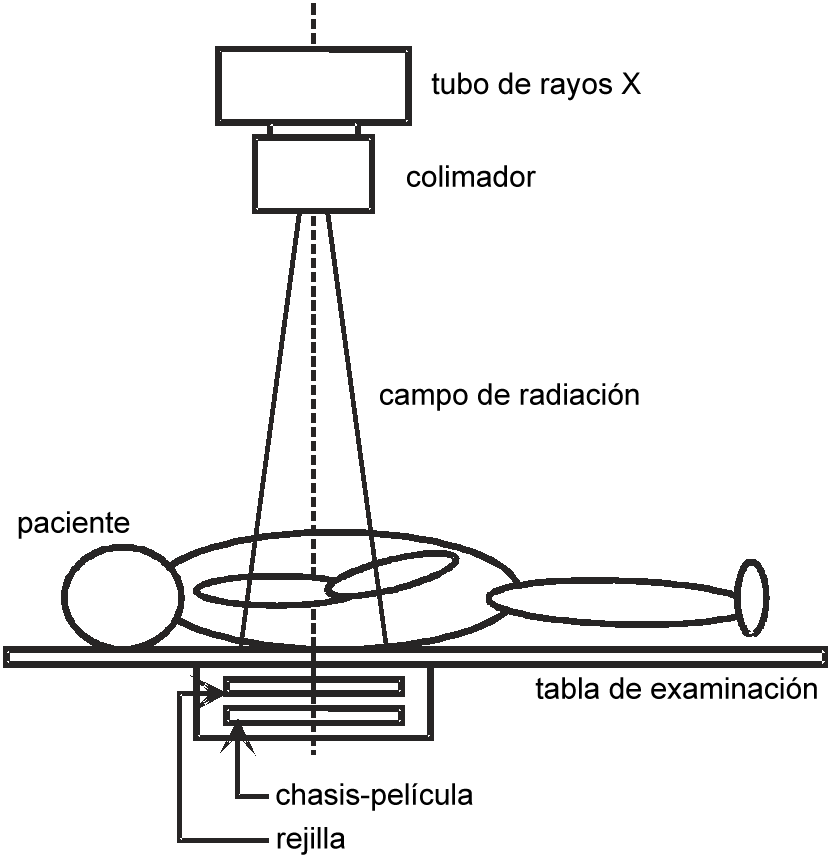
\includegraphics[width=0.40\columnwidth]{images/xray.png}
		\caption{Esquema de un examen de Rayos-X}
	\label{fig:xray}
\end{figure}

La imagen resultante es una proyecci\'on de una estructura tridimensional en un plano bidimensional. Como resultado de ello, pueden existir otras estructuras en el camino de la influencia del haz de Rayos-X y la toma. Esto genera la presencia de superficies solapadas u ocultas tales que complican la detecci\'on de la fractura, por lo que es necesario capturar im\'agenes desde m\'as de un punto de vista. Una vez que se obtiene un n\'umero suficiente de puntos de vista del hueso fracturado, las im\'agenes son analizadas por un radi\'ologo para determinar el lugar y forma de la fractura en el hueso. 

Dos tipos de proyecciones utilizadas muy frecuentemente son la proyecci\'on AP (anteroposterior) y LAT (lateral). La proyecci\'on AP consiste en colocar el paciente mirando hacia el equipo de Rayos-X \'o con una rotaci\'on de 180 grados con respecto a este. Por otro lado, la proyecci\'on LAT consiste en colocar al paciente con un giro de $\pm$ 90 grados con respecto a la parte frontal del equipo. En la Figura \ref{fig:proyeccionAP} se observa una placa de Rayos-X tomada a un t\'orax en una proyecci\'on AP, y en la Figura \ref{fig:proyeccionLAT} se observa el mismo t\'orax en una proyecci\'on LAT.

\begin{figure}[htb]
  \begin{center}
    \subfigure[]{\label{fig:proyeccionAP}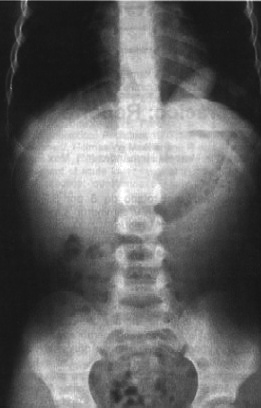
\includegraphics[width=0.20\columnwidth]{images/AP.png}} \hspace{1cm}
    \subfigure[]{\label{fig:proyeccionLAT}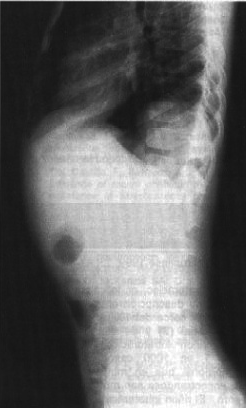
\includegraphics[width=0.20\columnwidth]{images/LAT.png}}
  \end{center}
  \caption{Rayos-X de un t\'orax abdominal simple en proyecci\'on (a) anteroposterior y (b) lateral}
  \label{fig:proyeccion}
\end{figure}

De acuerdo a \cite{SQUIRE69}, las im\'agenes de Rayos-X no son f\'aciles de examinar ya que se requiere de una buena interpretaci\'on de la misma para realizar un diagn\'ostico. Esto incluye tener un conocimiento sobre el lugar donde aparecen las sombras y la intensidad de las mismas de acuerdo a la posici\'on en el momento de la adquisici\'on de la imagen, para as\'i determinar con precisi\'on las caracter\'isticas de la fractura. Adicionalmente, se necesita una habilidad para recrear en 3D (geometr\'ia reconstructiva y espacial) a un paciente mientras se observa una imagen 2D. Finalmente, se analizan las sombras presentes con el objetivo de visualizar su estructura tridimensional y as\'i determinar una clasificaci\'on de la fractura.

%%%%%%%%%%%%%%%%%%%%%%%%%%%%%%%%%%%%%%%%%%%%%%%%
\subsection{Clasificaci\'on}

Una vez confirmada la presencia de una fractura, M\"{u}ller et al. \cite{MULL90} plantean que la lesi\'on en el hueso afectado debe ser reconocida, identificada y descrita utilizando la inspecci\'on de la imagen radiogr\'afica en concordancia con alg\'un esquema ya establecido. Existen diversos esquemas de fracturas, a continuaci\'on se mencionan algunos de ellos:

%%%%%%%%%%%%%%%%%%%%%%%%%%%%%%%%%%%%%%%%%%%%%%%%
\subsubsection{Esquema Salter-Harris}

La clasificaci\'on de Salter-Harris es utilizada principalmente para fracturas tratadas dentro del \'area de pediatr\'ia donde se utiliza una placa de crecimiento (met\'afisis). Este tipo de lesiones es aproximadamente el 15-20\% de las fracturas de f\'emur y tibia y 34\% de las fracturas de mano durante la infancia, seg\'un las estad\'isticas mostradas en \cite{UZE06}. La gran mayor\'ia de estas fracturas se curan sin ninguna alteraci\'on del mecanismo de crecimiento. En este esquema las fracturas son categorizadas en 5 tipos, los cuales se muestran en la Figura \ref{fig:SalterHarris} y se describen en la Tabla \ref{tab:fract}.

\begin{table}[htp]
\center
\begin{tabular}{|c|c|l|}
\hline
Tipo & Frecuencia & Descripci\'on \\ \hline
I & 5\% & Deslizamiento de la fisis \\ 
II & 75\% & Lesi\'on de la met\'afisis y de la fisis \\ 
III & 10\% & Lesi\'on de la ep\'ifisis y de la fisis \\ 
IV & 10\% & Lesi\'on de la met\'afisis, fisis y ep\'ifisis \\ 
V & < 1\% & Lesi\'on por compresi\'on de la fisis (aplastamiento) \\ 
\hline
\end{tabular}
\caption{Descripci\'on  de las categor\'ias del esquema Salter-Harris}
\label{tab:fract}
\end{table}

\begin{figure}[htb]
	\centering
		\includegraphics[width=1.0\columnwidth]{images/SalterHarris2.png}
		\caption{Tipos de fracturas bajo el esquema Salter-Harris}
	\label{fig:SalterHarris}
\end{figure}

%%%%%%%%%%%%%%%%%%%%%%%%%%%%%%%%%%%%%%%%%%%%%%%%
\subsubsection{Esquema Gustilo}

La clasificaci\'on de Gustilo \cite{BROW03} es para fracturas abiertas y est\'a basada en el grado de lesi\'on de las partes blandas. Esta clasificaci\'on plantea 3 grandes grupos que indican la cantidad de tejido blando da\~nado que es asociado con la fractura. La Tabla \ref{tab:gustilo} muestra la descripci\'on de cada uno de estos grupos.

\begin{table}[htp]
\center
\begin{tabular}{|c| p{13cm}|}
\hline
Grupo & Descripci\'on \\ \hline
1 & La herida es peque\~na, generalmente puntiforme, con escasa contusi\'on o deterioro de las partes blandas (piel, celular, m\'usculos, etc.). El traumatismo es de baja energ\'ia. \\
\hline
2 & La herida es amplia y la exposici\'on de las partes blandas profundas es evidente, pero el da\~no f\'isico de ellas es moderado. El traumatismo es de mediana energ\'ia. \\
\hline
3 & La herida es de gran tama\~no en extensi\'on y profundidad: a nivel cut\'aneo, celular y muscular. Generalmente hay da\~no importante de estructuras neuro-vasculares. El traumatismo es de alta energ\'ia. \\ 
\hline
\end{tabular}
\caption{Descripci\'on  de los grupos del esquema Gustilo}
\label{tab:gustilo}
\end{table}

%%%%%%%%%%%%%%%%%%%%%%%%%%%%%%%%%%%%%%%%%%%%%%%%
\subsubsection{Esquema Tscherne}

La clasificaci\'on de Tscherne \cite{STAN07} fue dise\~nada en 1982 y es s\'olo para fracturas cerradas. Se basa en un concepto subjetivo sobre la condici\'on general de la lesi\'on hecha con observaci\'on del m\'edico, conocimiento del mecanismo de la lesi\'on y la severidad de la fractura. Se basa en 4 grados de severidad: Grado 0, 1, 2 y 3. El nivel de severidad Grado 0 implica un da\~no m\'inimo sobre el tejido blando, causado por violencia indirecta y un patr\'on simple. Por otra parte, el nivel de severidad Grado 3 define una contusi\'on severa sobre el tejido, destrucci\'on del m\'usculo, lesiones vasculares, etc., causado por un impacto de alta energ\'ia.

%%%%%%%%%%%%%%%%%%%%%%%%%%%%%%%%%%%%%%%%%%%%%%%%
\subsubsection{Esquema AO}

Actualmente, la clasificaci\'on AO (siglas en alem\'an para \textit{Arbeitsgemeinschaft f\"{u}r Osteosynthesefragen}) para fracturas, es la clasificaci\'on m\'as aceptada internacionalmente. Se basa en clasificar la fractura de acuerdo a su ubicaci\'on y caracter\'istica morfol\'ogica. Seg\'un este esquema, se requiere de 4 letras/n\'umeros para ubicar con gran precisi\'on una fractura y su severidad (sin tomar en cuenta los subgrupos y la escala de severidad). 

La ubicaci\'on es asignada por dos n\'umeros, como se muestra en la Figura \ref{fig:AO}, que indica en cu\'al hueso y en cu\'al segmento ocurri\'o la fractura. La Tabla \ref{tab:AO} muestra la clasificaci\'on para los huesos.
\begin{table}
\begin{center}
\begin{tabular}{|c|l|}
\hline
Clasificaci\'on & Hueso \\ \hline
1 & H\'umero\\ 
2 & Radio/C\'ubito\\ 
3 & F\'emur/R\'otula\\ 
4 & Tibia/Peron\'e\\ 
5 & Columna vertebral\\ 
6 & Pelvis/Acetabular\\ 
7 & Huesos de la mano\\
8 & Huesos del pie\\ 
9 & Huesos craneomaxilofaciales\\ 
\hline
\end{tabular}	
%\caption{none}
\end{center}
\caption{Numeraci\'on de los huesos seg\'un el esquema de clasificaci\'on AO}
\label{tab:AO}
\end{table}


\begin{figure}[htb]
	\centering
		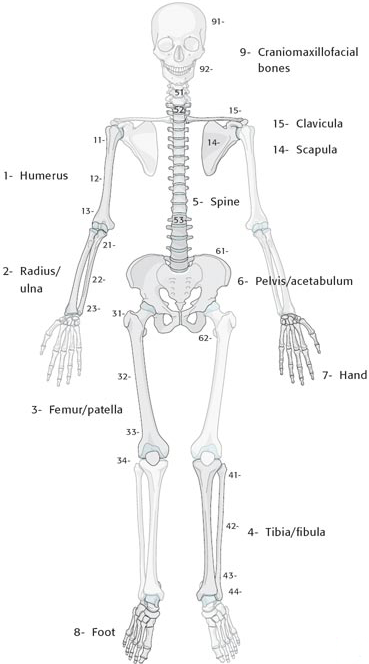
\includegraphics[width=0.35\textwidth]{images/ao_classification.png}
		\caption{Clasificaci\'on AO para la numeraci\'on de acuerdo a la ubicaci\'on anat\'omica de la fractura. Informaci\'on tomada de \cite{REF_AO}}
	\label{fig:AO}
\end{figure}

Esta notaci\'on alfanum\'erica sirve como gu\'ia al cirujano para la valoraci\'on de la fractura con una alta precisi\'on. Los huesos largos, se dividen en tres segmentos: 1=proximal, 2=di\'afisis y 3=distal. Una vez seleccionados ambos n\'umeros, entra en una clasificaci\'on por tipo de fractura (A=simple, B=en cu\~na y C=compleja). Luego, la fractura es dividida en tres grupos que miden la escala de severidad de la misma (1,2,3). En la Figura \ref{fig:AOfemur} se muestra la clasificaci\'on AO para el f\'emur en segmento diafisial.
\begin{figure}[htb]
	\centering
		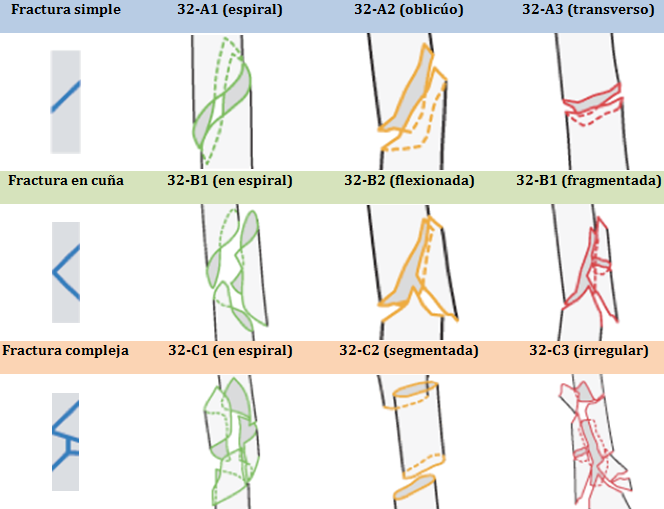
\includegraphics[width=0.7\textwidth]{images/ao_femur.png}
		\caption{Clasificaci\'on AO que corresponde a una fractura tipo 32}
	\label{fig:AOfemur}
\end{figure}

El esquema de clasificaci\'on de AO es recomendado por M\"{u}ller et. al. \cite{MULL90} al definirlo como una clasificaci\'on cl\'inicamente relevante, simple, reproducible y proporciona una buena estimaci\'on de los resultados cl\'inicos.

%%%%%%%%%%%%%%%%%%%%%%%%%%%%%%%%%%%%%%%%%%%%%%%%
\subsubsection{Otros esquemas}

Se pueden encontrar otros esquemas de clasificaci\'on que dependen exclusivamente del lugar de la lesi\'on. Seg\'un Koval y Zuckerman \cite{KOV02}, las fracturas de la pelvis pueden ser clasificadas bajo el esquema de Young y Burgess, las fracturas de la clav\'icula con la clasificaci\'on de Allman y las fracturas de la meseta tibial con la clasificaci\'on de Schatzker. Estas clasificaciones s\'olo son relevantes para su particular regi\'on anat\'omica, por lo que no pueden ser comparadas con las dem\'as que pueden ser aplicadas a todo el cuerpo humano.

%%%%%%%%%%%%%%%%%%%%%%%%%%%%%%%%%%%%%%%%%%%%%%%%
\subsection{Tratamiento}

Una fractura de hueso sana naturalmente a trav\'es de un proceso fisiol\'ogico siempre que se encuentre lo suficientemente inmovilizado. La insuficiente inmovilizaci\'on puede resultar en una cicatrizaci\'on inadecuada del hueso, y la formaci\'on de una pseudoartrosis. En consecuencia,  existen tres opciones principales para tratamiento en la reparaci\'on de fracturas de huesos, planteadas en \cite{MORO99}, donde todas requieren la inmovilizaci\'on de las piezas \'oseas fracturadas. 

Para tratar una fractura se efect\'ua un proceso de \textit{reducci\'on} que consiste en colocar los fragmentos de hueso en su alineaci\'on correcta. En las fracturas simples, el m\'etodo m\'as com\'un es la reducci\'on cerrada bajo anestesia, seguida por la aplicaci\'on de un yeso alrededor del exterior de la extremidad.

En fracturas m\'as severas, se emplea la reducci\'on abierta de la fracturas y la fijaci\'on interna (ver Figura \ref{fig:AOfijador}(a)). Esta t\'ecnica consiste en una cirug\'ia para colocar barras de metal, tornillos o placas por debajo de la piel y as\'i permitir que el hueso sane.
\begin{figure}[htb]
	\centering
		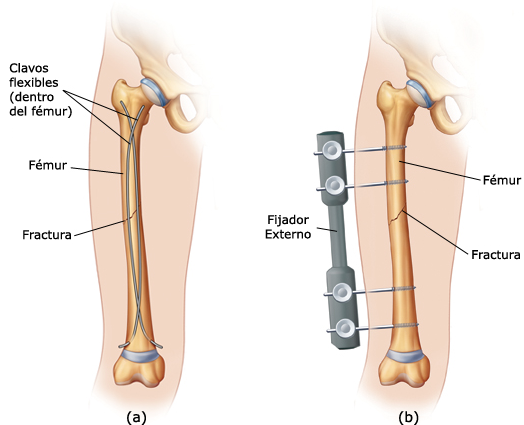
\includegraphics[width=0.55\textwidth]{images/fijadores.png}
		\caption{Inmovilizaci\'on de una fractura por (a) fijaci\'on interna y (b) fijaci\'on externa}
	\label{fig:AOfijador}
\end{figure}

Este procedimiento se recomienda para las fracturas complicadas que no se pueden reducir por bastidor, o en los casos en que el uso a largo plazo de una f\'erula no es recomendable. Por ejemplo, para las fracturas diafisiarias femorales donde se utiliza una placa, \'esta debe ser anat\'omica y su fijaci\'on debe quedar garantizada y es por ello que se emplean tornillos. Al mismo tiempo, un tratamiento de enclavado endomedular tambi\'en puede ser aplicado para este tipo de fracturas ya que tratan con \'exito la mayor parte de estas fracturas ya sean de trazo transversal, oblicuo, espiroideo, segmentario o conminuto.

Por \'ultimo, la reducci\'on de fracturas abiertas y fijaci\'on externa (ver Figura \ref{fig:AOfijador}(b)) consiste en una cirug\'ia para reparar la fractura y la colocaci\'on de un dispositivo de fijaci\'on externa en la extremidad con la fractura. Este dispositivo es un marco externo que sostiene los huesos y los mantiene en su posici\'on correcta mientras se curan. Esta t\'ecnica se aplica generalmente a las fracturas complejas que no pueden ser reparadas mediante reducci\'on abierta y fijaci\'on interna.

%%% End: 